\documentclass{standalone}
\usepackage{tikz}
\usepackage{siunitx}
\usetikzlibrary{shapes, patterns, decorations.pathmorphing}

\begin{document}
\begin{tikzpicture}

% Define colors - back to original colors
\definecolor{bedrock}{RGB}{120, 120, 120}
\definecolor{regolith}{RGB}{180, 150, 120}
\definecolor{ice}{RGB}{180, 220, 255}
\definecolor{sunlight}{RGB}{255, 215, 0}
\definecolor{shadow}{RGB}{40, 40, 60}
\definecolor{moonGray}{RGB}{180,180,180}
\definecolor{craterGray}{RGB}{120,120,120}
\definecolor{spaceBlue}{RGB}{10,10,40}

% White background with rim
\fill[white] (-1.5,-2.5) rectangle (8.5,2.5);

% Left side - Moon with polar region
\begin{scope}[xshift=1.5cm, yshift=0.25cm]
    \begin{scope}
        \clip (0,0) circle (1.4);
        \node[opacity=1] at (0,0) {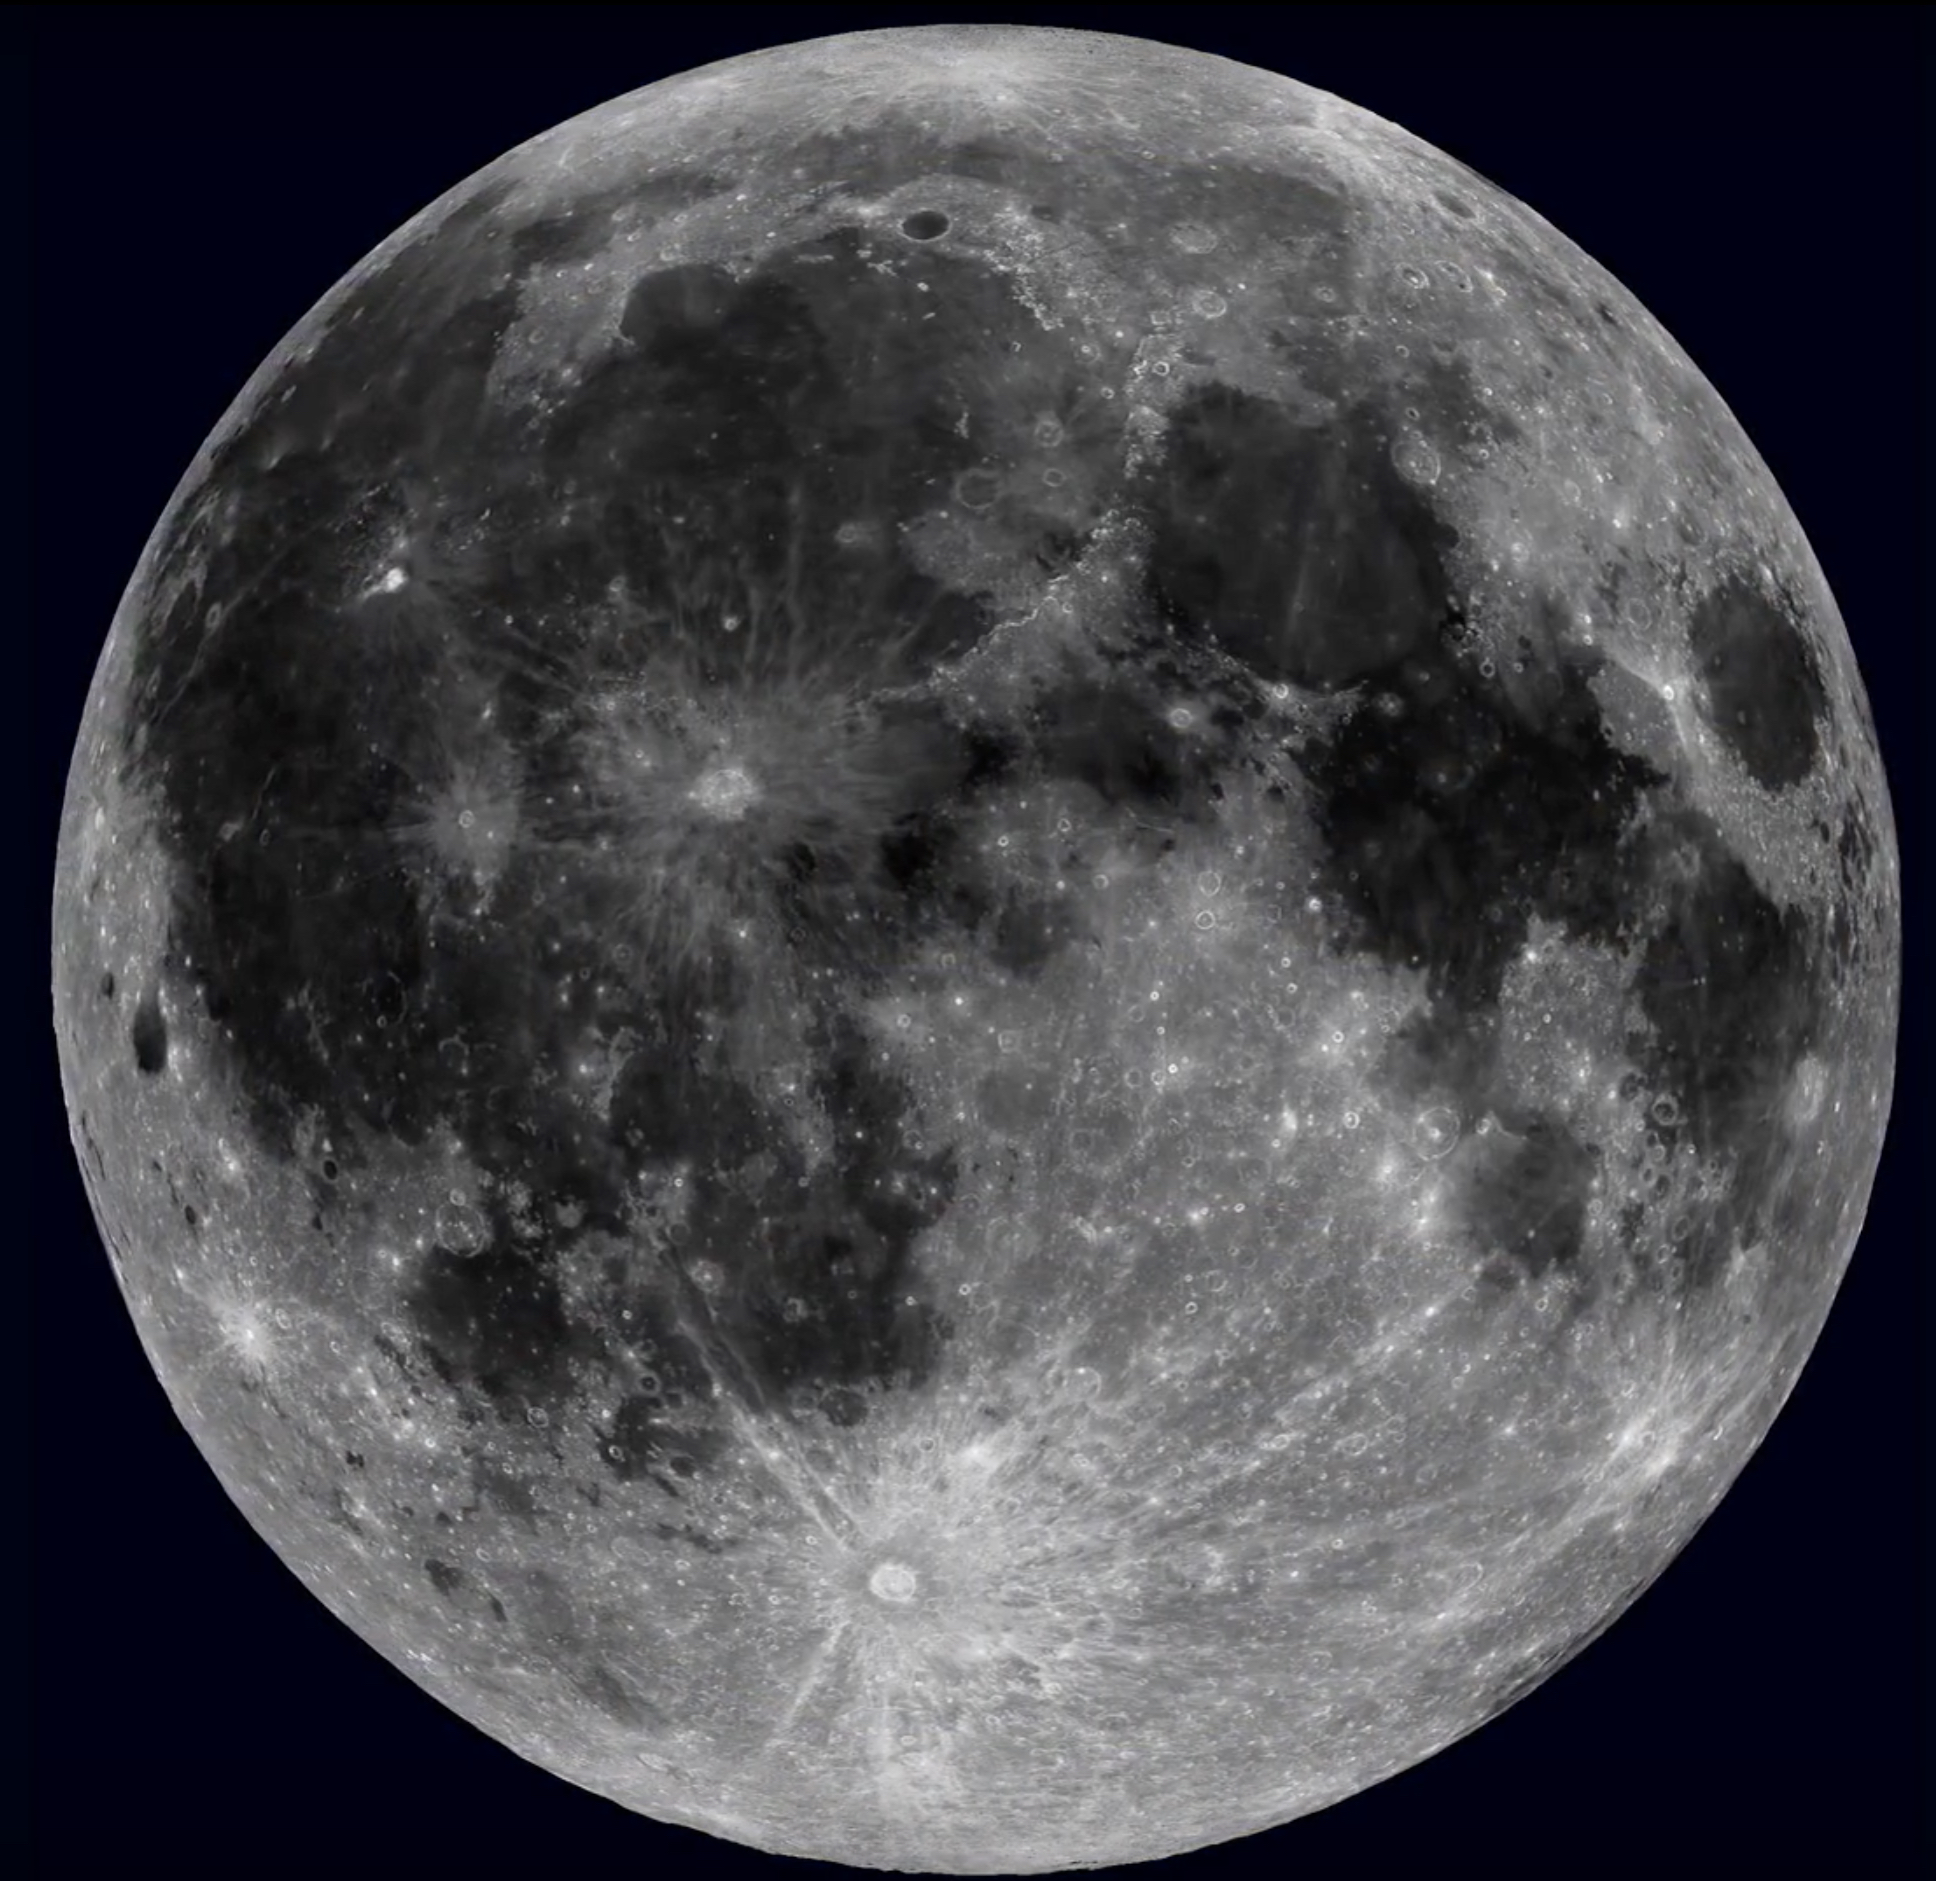
\includegraphics[width=3cm]{textures/lunar_nearside.jpg}};
    \end{scope}
    
    % Sun rays - parallel from the left
    \foreach \y in {-1.5,-1,-0.5,0,0.5,1,1.5} {
        \draw[sunlight, thick, ->] (-2.5,\y) -- (-1.5,\y);
    }
    
    % Magnifier focusing on north pole
    \fill[white, opacity=0.3] (0.1,1.4) circle (0.3);
    \draw[thick, black] (0.1,1.4) circle (0.3);
    \draw[thick, black] (0.1,1.4) circle (0.28);
    
    % Magnifier handle with grip
    \draw[thick, black, line cap=round] (0.3,1.2) -- (1.0,0.5);
    \draw[thick, black, line cap=round] (0.35,1.25) -- (1.05,0.55);
    \draw[thick, black, line cap=round] (1.0,0.5) -- (1.05,0.55);
    
    % Magnifier reflection/highlight
    \draw[white, thick, opacity=0.7] (0.0,1.5) arc (135:225:0.15);
    
\end{scope}

% Right side - Detailed cross-section of permanently shadowed crater
\begin{scope}[xshift=5cm, yshift=-1cm]
    % Bedrock base (thicker)
    \fill[bedrock] (0,0) rectangle (4,2.4);
    
    % Regolith layer (thinner) on top of ice
    \fill[regolith] (0,2.4) rectangle (4,2.5);
    
    % Crater shape - permanently shadowed (much deeper)
    \draw[thick] (1,2.5) .. controls (2,0.3) .. (3,2.5);

    % Ice layer following crater shape (thicker)
    \fill[ice] (1.3,2.5) .. controls (2,0.3) .. (2.7,2.5) .. controls (2.5,1.5) .. (1.5,1.5) -- cycle;

    % regolith layer on top of ice layer (thicker)
    \fill[regolith] (1,2.5) .. controls (2,0.7) .. (3,2.5) -- (3,2.5) -- (1,2.5) -- cycle;
    
    % Thicker regolith layer following crater shape (on top of ice)
    \fill[regolith!70] (1,2.5) .. controls (2,1.2) .. (3,2.5) -- (3,2.5) -- (1,2.5) -- cycle;

    % Solar ray from top left hitting crater rim
    \draw[sunlight, very thick, ->] (0.5,3.25) -- (2.5,1.75);
    \draw[sunlight, very thick, ->] (0,3.25) -- (1,2.5);
    \draw[sunlight, very thick, ->] (-0.5,3.25) -- (0.5,2.5);
    
    % Shadow area inside crater (darker overlay)
    \fill[shadow, opacity=0.4] 
    (1,2.5) -- % Crater rim where shadow starts
    (2.55,1.45) -- % Shadow line based on solar ray angle
    (2.55,1.45) .. controls (1.9,0.5) and (1.9,0.5) .. (1,2.5); % Follow crater curve back

    % Rock fragments in regolith
    \fill[bedrock] (0.3,2.3) -- (0.4,2.25) -- (0.5,2.35) -- (0.45,2.45) -- (0.35,2.4) -- cycle;
    \fill[bedrock] (0.8,2.35) -- (0.9,2.3) -- (1.0,2.4) -- (0.95,2.45) -- (0.85,2.42) -- cycle;
    \fill[bedrock] (3.2,2.3) -- (3.3,2.25) -- (3.4,2.35) -- (3.35,2.45) -- (3.25,2.4) -- cycle;
    
    % Surface texture
    \draw[decorate, decoration={random steps, segment length=2pt, amplitude=1pt}] (0,2.5) -- (1,2.5);
    \draw[decorate, decoration={random steps, segment length=2pt, amplitude=1pt}] (3,2.5) -- (4,2.5);
    
    % Labels
    \node at (2,-0.5) {\textbf{Permanently Shadowed Region}};
    \node at (2,-0.8) {Water ice preservation};
\end{scope}

\end{tikzpicture}
\end{document}